\documentclass[journal]{IEEEtran} % use the `journal` option for ITherm conference style
\IEEEoverridecommandlockouts
% The preceding line is only needed to identify funding in the first footnote. If that is unneeded, please comment it out.
\usepackage{cite}
\usepackage{amsmath,amssymb,amsfonts}
\usepackage{algorithmic}
\usepackage{graphicx}
\usepackage{textcomp}
\usepackage{xcolor}
\graphicspath{ {./images/} }
\def\BibTeX{{\rm B\kern-.05em{\sc i\kern-.025em b}\kern-.08em
    T\kern-.1667em\lower.7ex\hbox{E}\kern-.125emX}}
\begin{document}

\title{LIDAR Object Tracking with Hardware Acceleration}


\author{%%%% author names
    \IEEEauthorblockN{McCain Boonma}\\% first author
    \IEEEauthorblockA{\textit{Northeastern University, Boston, USA}}\\% first affiliation
    \IEEEauthorblockA{boonma.m@northeastern.edu}
}

\maketitle

\begin{abstract}
This project presents an efficient solution for real-time processing and analysis of LiDAR data, leveraging FPGA-based hardware acceleration to perform clustering and a Kalman filter for object tracking. Utilizing a YDLIDAR X4 LiDAR sensor, distance data is collected and processed to identify clusters representing objects within the field of view. A PYNQ overlay is employed to accelerate clustering operations on a Xilinx FPGA platform, significantly improving the overall performance. The integration of a  Kalman filter enables tracking of detected clusters over time, allowing for the identification and monitoring of objects with constant velocities. Visualization of the processed data is achieved using polar plots with the Matplotlib library, providing a clear representation of the raw LiDAR data and the identified clusters.
\end{abstract}

\section{Introduction}
Light Detection and Ranging (LiDAR) sensors are widely used in various applications, including autonomous vehicles, robotics, and environmental monitoring. These sensors generate large amounts of data that require real-time processing to detect and track objects within their field of view. This paper presents an efficient solution for real-time processing and analysis of LiDAR data, leveraging FPGA-based hardware acceleration to perform clustering and a Kalman filter for object tracking. The proposed approach employs a number of hardware optimizations in the point clustering operation, resulting in significant improvements in overall performance. The processed data is visualized using polar plots , providing a clear representation of the raw LiDAR data and the identified clusters.

\section{System Overview}
This inclusive system (Fig \ref{fig:sysOverview}) includes LIDAR data collection, point clustering, and object tracking. The primary focus of this paper is the clustering algortihm implemented on the FPGA programmable logic via an overlay and the object tracking using a Kalman filter implemented on the FPGA processing system. 

\begin{figure}[h]
  \centering
  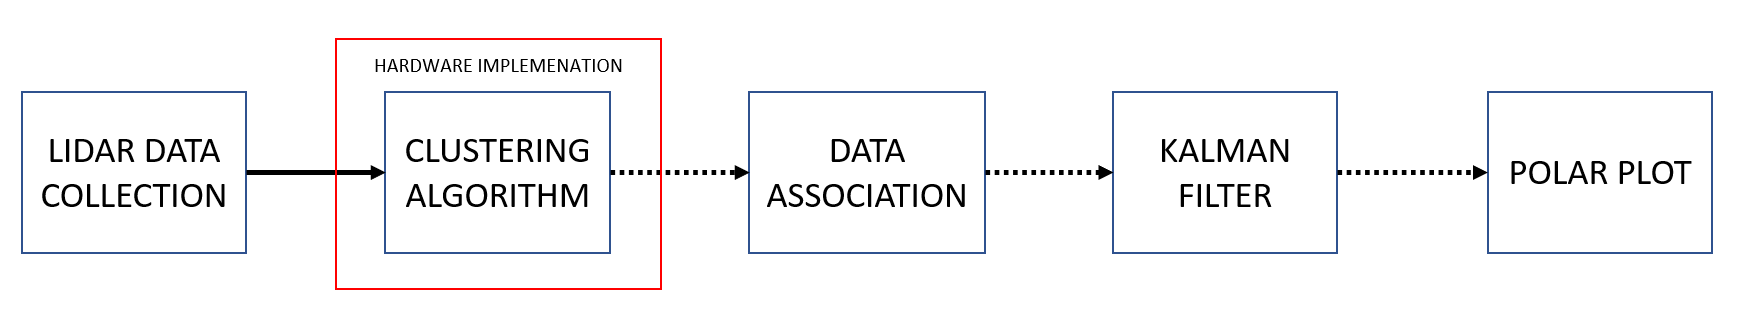
\includegraphics[width=0.5\textwidth]{sysOverview}
  \caption{System Overview}
  \label{fig:sysOverview}
\end{figure}

\subsection{LiDAR Data Collection}

The sensor's coordinate system is defined such that 0\textdegree originates from the center of the sensor assembly towards the LIDAR sensor's motor, with data collected in the clockwise direction (as shown in Fig. \ref{fig:polarLIDAR}). The sensor is connected to the processing system of the PYNQ Z2 via a USB port.

\begin{figure}[h]
  \centering
  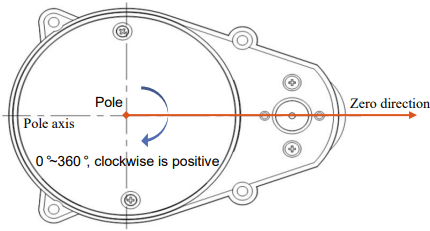
\includegraphics[width=0.35\textwidth]{polarLIDAR}
  \caption{LIDAR Sensor Coordinate System Definition}
  \label{fig:polarLIDAR}
\end{figure}

 To control the LIDAR sensor and collect LIDAR data, the PyLidar3 library is utilized, which is a python 3 package. The LIDAR sensor is capable of a typical angle resolution of 0.50\textdegree at 7 Hz, but due to software limitations, the PyLidar3 library provides a resolution of only 1\textdegree regardless of the frequency. The collected data is returned in the form of a dictionary, comprising of 360 degrees of angle and corresponding distances in millimeters.\\


\subsection{Hardware Accelerated Point Clustering}

The point clustering operation was implemented on the programmable logic of the FPGA using an Overlay. To achieve this, the point clustering algorithm was developed in Vitis High-Level Synthesis (HLS). The LIDAR data is transferred from the FPGA processing system to the programmable logic through an AXI Stream interface, while the clustered data is transferred via a separate AXI Stream interface. The implemented clustering algorithm is based on the Density-Based Spatial Clustering of Applications with Noise (DBSCAN) algorithm, which is commonly utilized in LIDAR point clustering applications.\\

he clustering algorithm utilized in the proposed LIDAR object tracking system is based on the Density-Based Spatial Clustering of Applications with Noise (DBSCAN) algorithm. The DBSCAN algorithm takes three parameters: an array of distance data, the number of data points, and the maximum distance between two points in the same neighborhood (epsilon, $\epsilon$).

The DBSCAN algorithm starts by iterating over all the points in the input data array. For each unvisited point, the algorithm finds all its neighbors within a distance of $\epsilon$ and adds them to a cluster. The algorithm then expands the cluster by adding all reachable neighbors of each point in the cluster. The algorithm stops when no more points can be added to the cluster.

The distance calculation used in the DBSCAN algorithm takes into account the angle between the LIDAR points, which are represented as distances in an array. Given two points $p_1$ and $p_2$ in the array, the distance calculation between them is as follows:

\begin{equation}
distance = \sqrt{(p_{1,x} - p_{2,x})^2 + (p_{1,y} - p_{2,y})^2}
\end{equation}

Where $p_{1,x}$ and $p_{2,x}$ are the distances of $p_1$ and $p_2$ from the LIDAR sensor along the horizontal axis, and $p_{1,y}$ and $p_{2,y}$ are the distances of $p_1$ and $p_2$ from the LIDAR sensor along the vertical axis. The distance calculation also involves converting the angles of the LIDAR points to radians, and using the sine and cosine functions to compute the horizontal and vertical distances respectively.

The implemented DBSCAN algorithm in the code snippet takes an array of distance data, the number of data points, and the maximum distance between two points in the same neighborhood (epsilon, $\epsilon$) as input. The algorithm iterates over all the points in the input array, finds all the neighbors of each unvisited point, and creates a new cluster if the point has enough neighbors. The algorithm then expands the cluster by adding all reachable neighbors, and continues until no more points can be added to the cluster.


\subsection{Constant Velocity Kalman Filter for Object Tracking [WORK IN PROGRESS]}

The Kalman filter is a mathematical algorithm that uses a series of measurements observed over time to estimate the state of a system. The Kalman filter is widely used in many applications, including control systems, navigation systems, and signal processing. The filter is based on a set of equations that describe the state of the system, the measurements, and the noise in the system.

The Kalman filter has two phases: the prediction phase and the update phase. In the prediction phase, the filter predicts the state of the system at the next time step based on the previous state and the control input. The prediction is then updated using the current measurement to improve the estimate of the system state. The filter uses a transition matrix, observation matrix, initial state mean, and initial state covariance to model the system.

The equations used in the code to initialize the Kalman filter are as follows:

\begin{equation}
\mathbf{x}_k = \begin{bmatrix} x_k \ y_k \ \dot{x}_k \ \dot{y}_k \end{bmatrix}
\end{equation}

\begin{equation}
\mathbf{F} = \begin{bmatrix} 1 & 0 & \Delta t & 0 \\ 0 & 1 & 0 & \Delta t \\ 0 & 0 & 1 & 0 \\ 0 & 0 & 0 & 1 \end{bmatrix}
\end{equation}

\begin{equation}
\mathbf{H} = \begin{bmatrix} 1 & 0 & 0 & 0 \ 0 & 1 & 0 & 0 \end{bmatrix}
\end{equation}

\begin{equation}
\mathbf{Q} = \begin{bmatrix} \sigma_x^2 & 0 & 0 & 0 \\ 0 & \sigma_y^2 & 0 & 0 \\ 0 & 0 & \sigma_{\dot{x}}^2 & 0 \\ 0 & 0 & 0 & \sigma_{\dot{y}}^2 \end{bmatrix}
\end{equation}

\begin{equation}
\mathbf{R} = \begin{bmatrix} \sigma_{\text{measurement}}^2 & 0 \ 0 & \sigma_{\text{measurement}}^2 \end{bmatrix}
\end{equation}

where $\mathbf{x}_k$ is the state vector at time step $k$, $\mathbf{F}$ is the state transition matrix, $\mathbf{H}$ is the observation matrix, $\mathbf{Q}$ is the process noise covariance matrix, and $\mathbf{R}$ is the measurement noise covariance matrix. The values of the matrices are initialized to appropriate values based on the specific application.

The Kalman filter is updated using the following equations:

\begin{equation}
\mathbf{x}{k|k-1} = \mathbf{F}\mathbf{x}{k-1|k-1}
\end{equation}

\begin{equation}
\mathbf{P}{k|k-1} = \mathbf{F}\mathbf{P}{k-1|k-1}\mathbf{F}^T + \mathbf{Q}
\end{equation}

\begin{equation}
\mathbf{K}k = \mathbf{P}{k|k-1}\mathbf{H}^T(\mathbf{H}\mathbf{P}_{k|k-1}\mathbf{H}^T + \mathbf{R})^{-1}
\end{equation}


\begin{equation}
\mathbf{x}{k|k} = \mathbf{x}{k|k-1} + \mathbf{K}_k(\mathbf{z}k - \mathbf{H}\mathbf{x}{k|k-1})
\end{equation}

where $\mathbf{P}_{k|k-1}$ is the predicted state covariance matrix, $\mathbf{K}_k$ is the Kalman gain matrix, and $\mathbf{z}_k$ is the measurement vector at time step $k$. These equations are used to update the Kalman filter estimate of the state at each time step.

In the code provided, the function init\_kalman\_filter() initializes the Kalman filter with the transition matrix, observation matrix, initial state mean, and initial state covariance. The kf.filter\_update() function is used to update the Kalman filter estimate based on the current measurement. The cluster\_states dictionary is used to store the mean state and covariance of each cluster over time. These values are updated at each time step using the Kalman filter update equations. Overall, the Kalman filter is used in the code to improve the accuracy of the distance and angle measurements obtained from the Lidar sensor.

\subsection{Data Association - Nearest Neighbor Algorithm - WORK IN PROGRESS}

Data association is an important step in object tracking to match the detected clusters in the current frame with the tracked objects from the previous frame. (STILL FIXING SOME MAJOR BUGS)

\subsection{Visualization}

Visualization plays a crucial role in analyzing the performance of the LiDAR data processing pipeline and understanding the identified clusters and their tracked positions. This project uses the Matplotlib library to generate polar plots for the visualization of raw LiDAR data, identified clusters, and tracked objects.

Two polar plots are created for each iteration of the processing loop:
\begin{itemize}

\item Raw Data Plot: This plot displays the distance values collected by the LiDAR sensor at different angles. It helps to visualize the raw LiDAR data and understand the environment.

\item Clustered Data Plot: This plot shows the identified clusters and their tracked positions, represented by red crosses. It is useful for evaluating the performance of the clustering algorithm and tracking filter.

\end{itemize}

The update\_plot function is responsible for updating the polar plots with the raw and clustered data. It first clears the axes, then plots the data points on the respective polar plots, and finally updates the plot titles and limits. The function also calls the data\_association function to perform data association between the current and previous clusters and update the state of the tracked objects in the constant velocity Kalman filter.

\section{Implementation}

\subsection{Hardware}
The clustering operation is an ideal candidate for hardware acceleration due to its computationally intensive nature and the ability to parallelize the algorithm. By grouping distances into clusters using a straightforward algorithm, hardware acceleration can significantly improve performance. The functionality of the clustering operation was verified by comparing the clusters generated by the hardware implementation to those generated by a software implementation using the same data.

\subsection{Software}
The Kalman Filter and data association are potential candidates for hardware acceleration. However, due to the intricacy of their mathematical algorithms and time constraints, hardware testing would have been excessively time-consuming. Thus, software implementation was chosen to expedite the development process.

\subsection{Implementation Overview}

The entire processing pipeline is implemented in a Jupyter Notebook, using the PYNQ library for FPGA acceleration, PyLidar3 library for LiDAR data collection, and the Matplotlib library for data visualization. The constant velocity Kalman filter is implemented using the pykalman library.

First, the LiDAR sensor is initialized and connected to the Linux-based system. Then, the PYNQ overlay is loaded onto the FPGA, and the input and output buffers are allocated for the clustering operation. The processing loop iterates for a user-defined number of times, performing the following steps in each iteration:

\begin{enumerate}
\item Collect distance data from the LiDAR sensor.
\item Perform the FPGA-based clustering operation on the collected data.
\item Update the constant velocity Kalman filter for the detected clusters.
\item Perform data association between the current and previous clusters.
\item Update the polar plots with the raw and clustered data.
\end{enumerate}

Upon completion of the processing loop, the LiDAR sensor is disconnected, and the program exits.


\section{Results and Discussion}

The proposed solution demonstrates the effectiveness of FPGA-based hardware acceleration for real-time processing and analysis of LiDAR data. By offloading the computationally intensive clustering operation onto the FPGA, the overall performance of the system is improved.

The polar plot visualization provides a clear representation of the raw LiDAR data and the identified clusters, facilitating the analysis of the system's performance. The data association algorithm successfully matches the detected clusters with the tracked objects, ensuring that the state of the constant velocity Kalman filter is updated correctly.

The data association portion of the project is currently facing major issues, rendering it non-operational (work is still ongoing to address these issues). Consequently, the Kalman filter is only able to return the current mean position of a cluster, and it is not yet behaving as a fully functional Kalman Filter. Despite these issues, communication between the LIDAR sensor and the PYNQ board is reliable, and connectivity issues are rare. While the clustering operation has not been benchmarked against the initial software implementation, it is operating reliably. However, plotting the data remains the slowest part of the pipeline.

Despite these challenges, the project is capable of connecting to a LIDAR sensor and successfully clustering LiDAR data. Additionally, groundwork has been laid for a functioning Kalman Filter, which will enable accurate tracking of objects with constant velocities.

\section{Conclusion}

This paper presents an efficient solution for real-time processing and analysis of LiDAR data using FPGA-based hardware acceleration. The proposed approach employs a YDLIDAR X4 LiDAR sensor for data collection and a Xilinx FPGA platform for acceleration, achieving significant improvements in overall performance. The integration of a constant velocity Kalman filter enables accurate tracking of detected clusters over time, while the data visualization using polar plots provides a clear representation of the raw LiDAR data and the identified clusters. Future work may explore the use of more advanced clustering algorithms and tracking filters to further enhance the performance of the system, as well as the implementation of additional features such as object classification and prediction.

\begin{thebibliography}{00}
    \bibitem{b1} L, Mallidi, "PyLidar3," GitHub, 2020, url: https://github.com/lakshmanmallidi/PyLidar3
    \bibitem{b2} K, Konstantinidis, "Detection and Tracking of Moving Objects with 2D LIDAR," GitHub, 2022, url: https://github.com/kostaskonkk/datmo
    \bibitem{b3} K. Beomseong, C. Baehoon, Y. Minkyun, K. Hyunju, K. Euntai. (2014). Robust Object Segmentation Using a Multi-Layer Laser Scanner. Sensors (Basel, Switzerland). 14. 20400-18. 10.3390/s141120400. 
    \bibitem{b4} R. Su, J. Tang, J. Yuan and Y. Bi, "Nearest Neighbor Data Association Algorithm Based on Robust Kalman Filtering," 2021 2nd International Symposium on Computer Engineering and Intelligent Communications (ISCEIC), Nanjing, China, 2021, pp. 177-181, doi: 10.1109/ISCEIC53685.2021.00044.
    \bibitem{b5} N. Baisa, "Derivation of a Constant Velocity Motion Model for Visual Tracking," arXiv, 2020, doi: 10.48550/ARXIV.2005.00844

\end{thebibliography}

\end{document}
